\documentclass{beamer}

\usetheme{Copenhagen}
\usepackage[utf8]{inputenc}
\usepackage{graphics}

% Slayt basliklarinda kullanilan font boyutu
\setbeamerfont{frametitle}{size=\normalsize}

\title{Resim İşleme}
\author{Nurettin Şenyer}
\date{Mart, 2011}
\institute[2011]{19/x}

\begin{document}

\frame{\titlepage}

\frame {
	\frametitle{İçindekiler}

	\begin{itemize}
		\item Resim Biçimlendirme
		\item Nokta ve Öbek İşleme
		\item İkil Resim İşleme
		\item Yansılar Pınar Duygulu, Alyosha Efros ve Shapiro ve Stockman'den
		uyarlanmıştır
	\end{itemize}
}

\frame {
	\frametitle{Resim İşleme}

	\begin{columns}
		\column{0.4\textwidth}
			\begin{itemize}
				\item ışık yüzeye düşer
				\item yüzey yansıtır/yutar
				\item sensör yansıyanı toplar
				\item yoğunluk (parlaklık,intensity) önemlidir
				\item açı önemlidir
				\item malzeme önemlidir
			\end{itemize}
		\column{0.6\textwidth}
			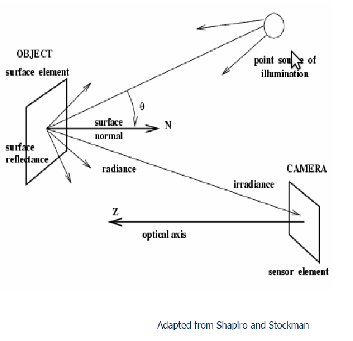
\includegraphics[width=0.9\textwidth]{img/03-form.png}
	\end{columns}
}

\frame {
	\frametitle{Resim Biçimlendirme: Sayısallaştırma}

	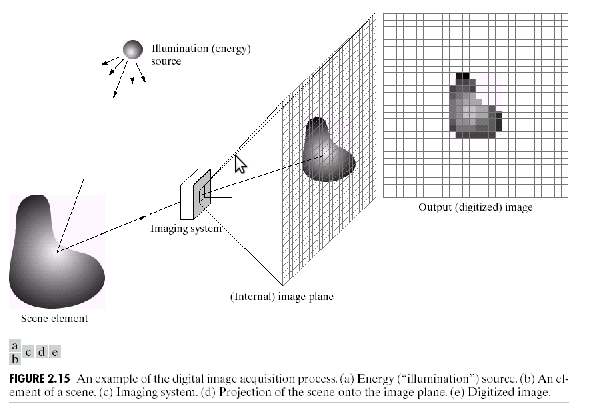
\includegraphics[width=0.9\textwidth]{img/04-form.png}
}

\frame {
	\frametitle{Örnekleme ve Nicemleme: Nyquist}

	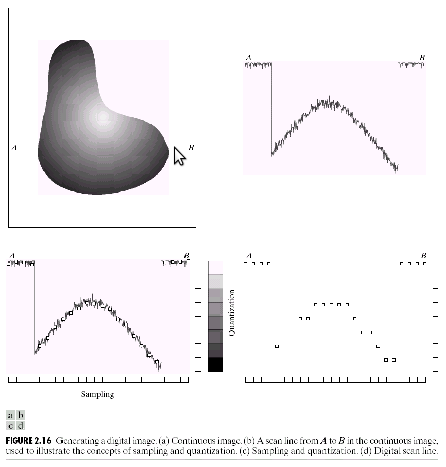
\includegraphics[width=0.9\textwidth]{img/05-samp.png}
}

\frame {
	\frametitle{Örnekleme ve Nicemleme}

	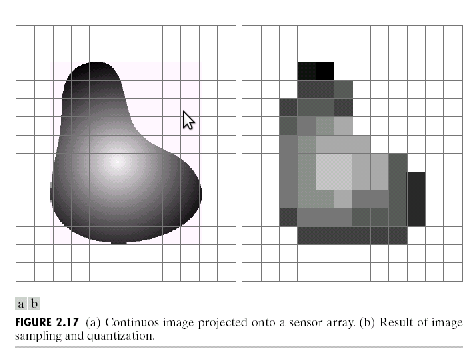
\includegraphics[width=0.9\textwidth]{img/06-quant.png}
}

\frame {
	\frametitle {Resim nedir?}

	\begin{itemize}
		\item $R^2$'den $R$'ye haritalama yapan $f$ işlevi olarak düşünelim
		\item $f(x, y)$ parlaklık değeri; $8 bit$ ise $0-255$ değerleri
		\item renkli ise vektör formu: $f(x,y) = [R(x,y) G(x,y) B(x,y)]$
	\end{itemize}
}

\frame {
	\frametitle{İşlev olarak Resim}

	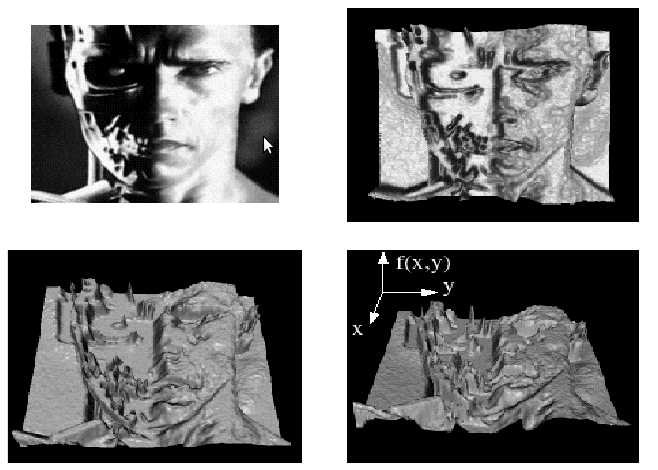
\includegraphics[width=0.9\textwidth]{img/08-img.png}
}

\frame {
	\frametitle{Sayısal Resim Nedir?}

	Örnekleme, nicemleme, ızgara etki, tamsayı değerler

	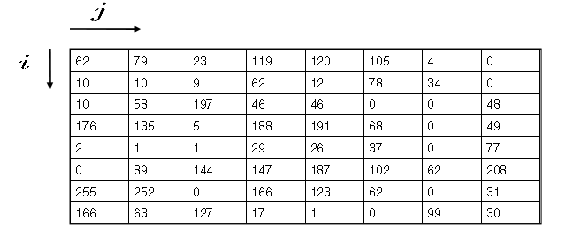
\includegraphics[width=0.9\textwidth]{img/09-matr.png}
}

\frame {
	\frametitle {Nokta İşleme}

	\begin{itemize}
		\item girdi: $f$ ve çıktı: $g$; $ g = T(f)$
		\item a) her bir pikseli bağımsız işle, piksel girdi/çıktı
		\item b) pikseli komşularıyla işle, tek piksel çıktı
		\item c) resmi işle, tek piksel/resim üret
	\end{itemize}
}
\frame {
	\frametitle{Noktasal İşleme}
	$g = f^\gamma$
	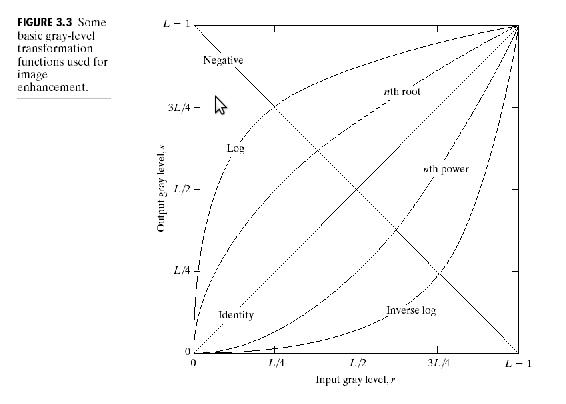
\includegraphics[width=0.9\textwidth]{img/11-gam.png}
}

\frame {
	\frametitle{Negatif}
	$g = -f$
	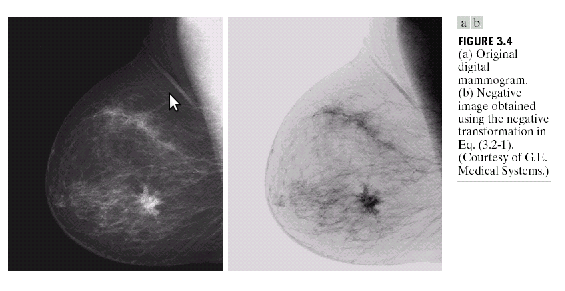
\includegraphics[width=0.9\textwidth]{img/12-neg.png}
}

\frame {
	\frametitle{İyileştirme}
	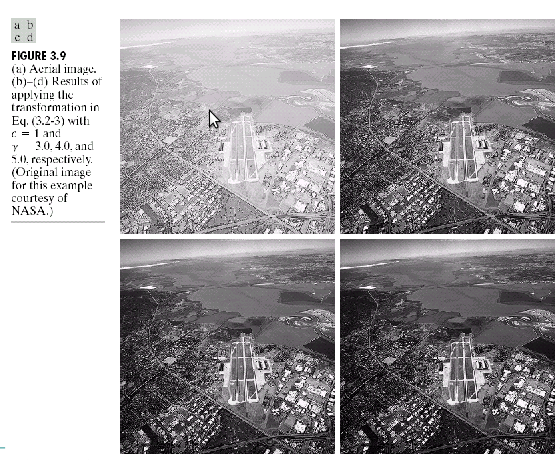
\includegraphics[width=0.9\textwidth]{img/13-enh.png}
}

\frame {
	\frametitle{Kontrast Yayma}
	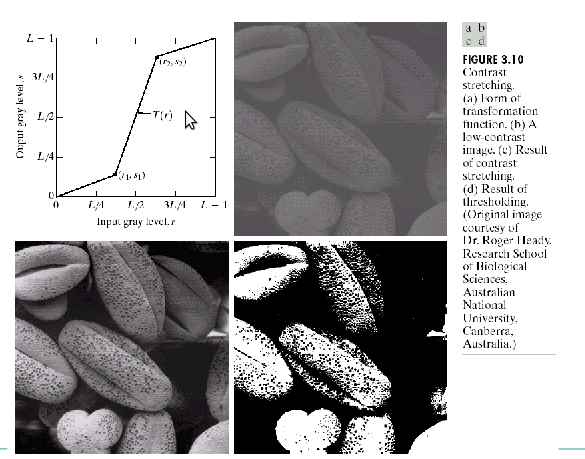
\includegraphics[width=0.9\textwidth]{img/14-str.png}
}

\frame {
	\frametitle{Histogram}
	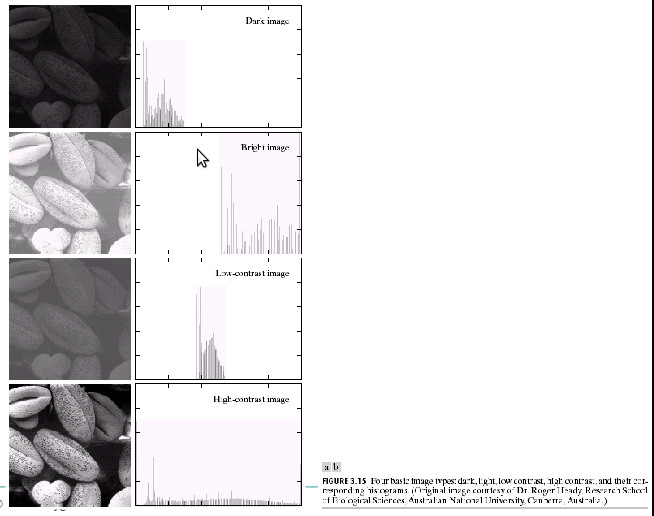
\includegraphics[width=0.9\textwidth]{img/15-hist.png}
}

\frame {
	\frametitle{Komşuluk İlişkisi}

	Resimdeki tüm pikseller karıştırılırsa ne olur?
	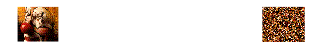
\includegraphics[width=0.9\textwidth]{img/16-neig.png}

	Histogramı aynıdır. Noktsal işlemden etkilenmez.
	\medskip
	Konumsal ilişki
}

\frame {
	\frametitle{Öbek (Blob) Çıkartma}
	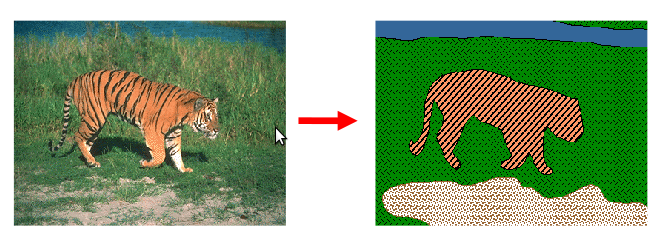
\includegraphics[width=0.9\textwidth]{img/17-blob.png}

	\begin{itemize}
		\item Blob: aralarında ilişki bulunan resim bölgesi
		\item nesne çıkarma, nesne silme, birleştirme vs
		\item genelde "blob" nesne değildir
	\end{itemize}
}
\frame {
	\frametitle{Blob Bağlılığı}
	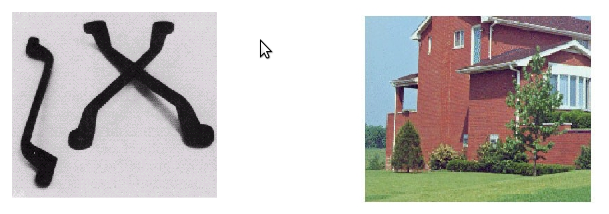
\includegraphics[width=0.9\textwidth]{img/18-coh.png}

	Takım, blob olabilir.
	Ev, çimen ve gökyüzü farklı bloblardır.
	`regionprops`, ikil resimlerde blob özniteliklerini çıkarır.
}
\frame {
	\frametitle{Blob'un Anlamı Nedir?}
	Resim, color/face/motion/edge detectorün çıkışı
	Şimdi Blob nedir? Yine, aralarında ilişki bulunan resim bölgeleri.

	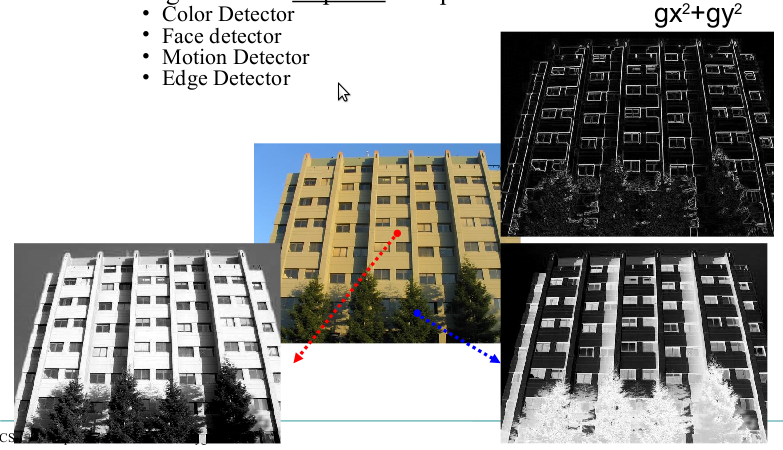
\includegraphics[width=0.9\textwidth]{img/19-edge.png}
}

\frame {
	\frametitle{Neden faydalıdır?}
	Resim
	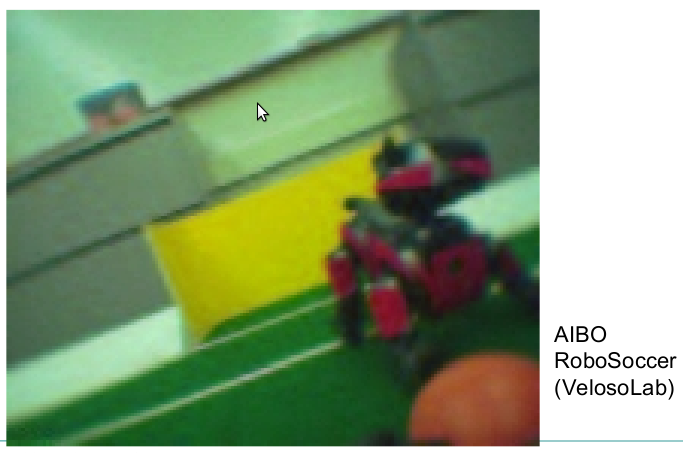
\includegraphics[width=0.9\textwidth]{img/20-ro.png}
}

\frame {
	\frametitle{İdeal Bölütleme}
	Color bölütleyici/detektör çıkışı
	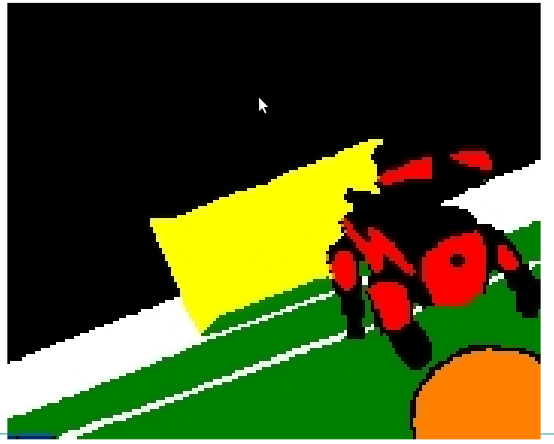
\includegraphics[width=0.9\textwidth]{img/21-seg.png}
}

\frame {
	\frametitle{Bölütleme Sonucu}
	Bloblar?
	\textbf{DEMO}: indirilen kodlar

	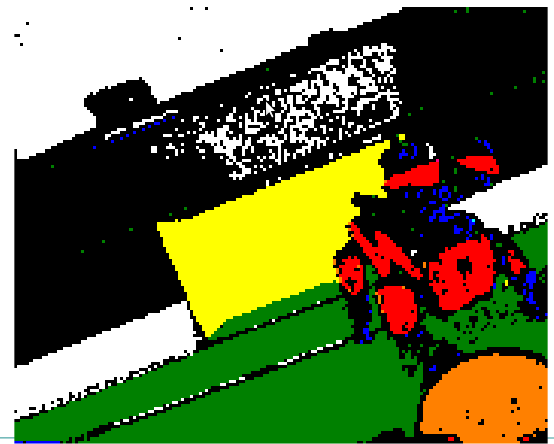
\includegraphics[width=0.9\textwidth]{img/22-seg.png}
}

\frame {
	\frametitle{Eşikleme}

	Temel eşikleme işlemi: $im(x,y) > T$ ise $bw(x,y) = 1$
	$T$ ne olacak? Otsu'nun yöntemi

	\begin{example}
		>> T = graythreshold(I); BW = im2bw(I, T);
	\end{example}

	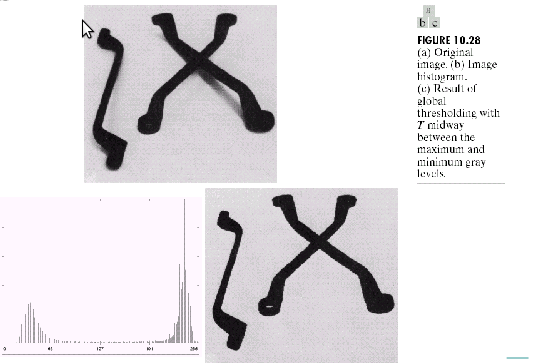
\includegraphics[width=0.9\textwidth]{img/23-th.png}
}

\frame {
	\frametitle{Kenar Algılama}

	Kenar algıla, sonra, Eşikle
	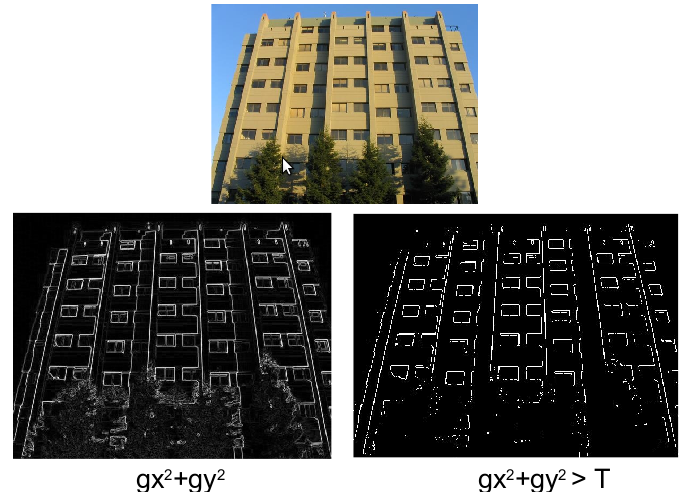
\includegraphics[width=0.9\textwidth]{img/24-edge.png}
}

\frame {
	\frametitle{Bazen iyi çalışır}

	Potansiyel problem... Gürültü...
	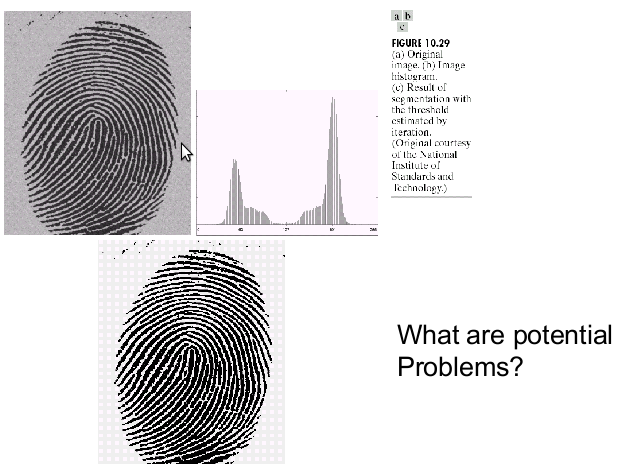
\includegraphics[width=0.9\textwidth]{img/25-fing.png}
}

\frame {
	\frametitle{... bazen de işe yaramaz}

	bu durumda da uyarlanır eşikleme
	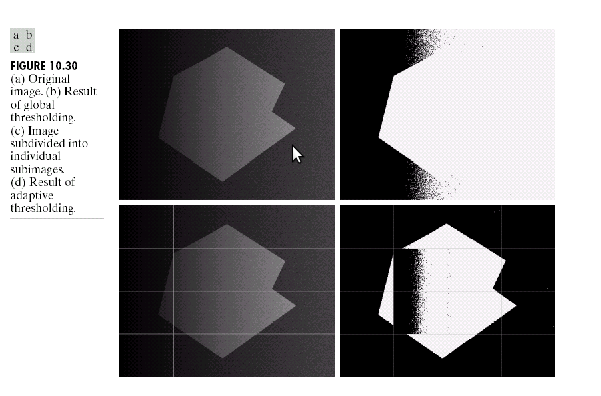
\includegraphics[width=0.9\textwidth]{img/26-adap.png}
}

\frame {
	\frametitle{Region Growing}
	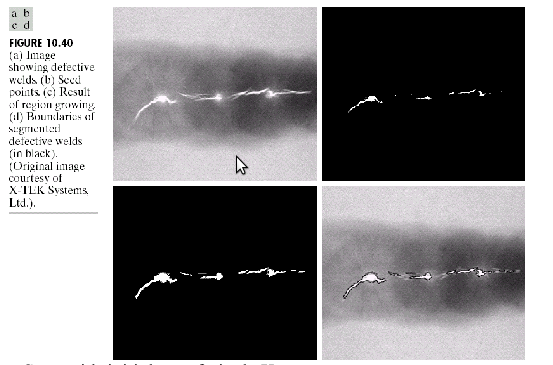
\includegraphics[width=0.9\textwidth]{img/27-region.png}
}

\frame {
	\frametitle{Region Growing}

	\begin{itemize}
		\item seed pikseli seç: $z_{seed}$ (ör.histogramdaki tepe noktası)

		\item komşu pikselleri denetle: $z$; eğer seed'e benziyorsa region'a
		ekle

		\item ::::: benzerlik (region membership criterion): ort.parlaklık,
		varyans, renk, doku, hareket, şekil/boyut, vs

		\item ::::: ör. $| z - z_{seed} | < T$

		\item region'a eklenen her bir piksel için 2. adımı yinele
	\end{itemize}

	DEMO: Region Growing
}

\frame {
	\frametitle{Renk temelli Blob Bölütleme}

	\begin{columns}
		\column{0.6\textwidth}
			\begin{itemize}
				\item $N$ renkle başla, $K$ renge in
				\item histogramdaki modlara bak
			\end{itemize}
		\column{0.4\textwidth}
			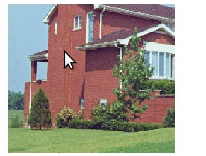
\includegraphics[width=0.9\textwidth]{img/28-color.png}
	\end{columns}
}

\frame {
	\frametitle{histogramdaki modları bulma}

	kaç mode var?
	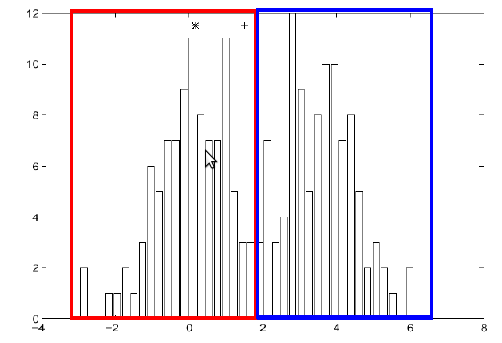
\includegraphics[width=0.9\textwidth]{img/29-hist.png}
}

\frame {
	\frametitle{Mean-shift (Comaniciu ve Meer)}

	parametrik olmayan öznitelik uzayı analiz tekniğidir.
	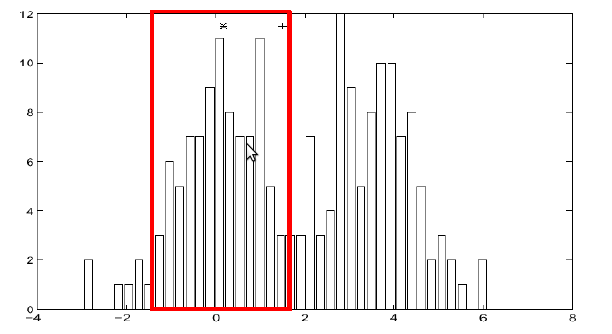
\includegraphics[width=0.9\textwidth]{img/30-mean.png}

	\begin{itemize}
		\item rastgele seed ve sabit boyutlu pencereyle başla
		\item pencerenin ağırlık merkezini hesapla ("mean")
		\item mean'e arama penceresini kaydır
		\item yakınsayıncaya kadar 2. adımı yinele
	\end{itemize}
}

\frame {
	\frametitle{Mean-shift (Comaniciu ve Meer)}
	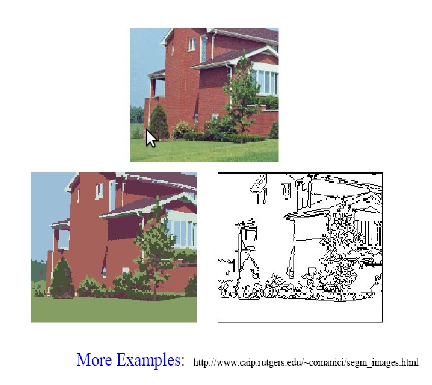
\includegraphics[width=0.9\textwidth]{img/31-mean.png}
	Bkz: `01comanivic.pdf`
}

\frame {
	\frametitle{Konular}

	Böylesi bir resmi nasıl idare edeceğiz?
	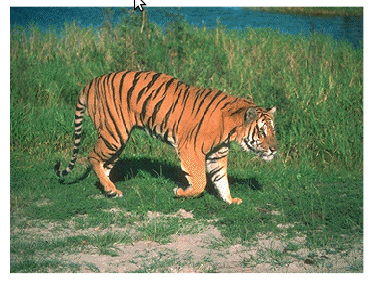
\includegraphics[width=0.9\textwidth]{img/32-iss.png}
	Mesele `blob != nesne`
}

\frame {
	\frametitle{İkil Resim İşleme}

	Şekilbilimsel Resim İşleme ...

	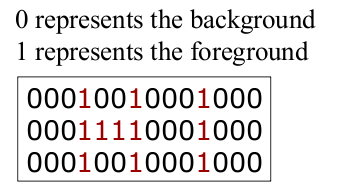
\includegraphics[width=0.9\textwidth]{img/33-bin.png}
}

\frame {
	\frametitle{Uygulama Alanları}

	Döküman analizi, endüstri, tıp, ...

	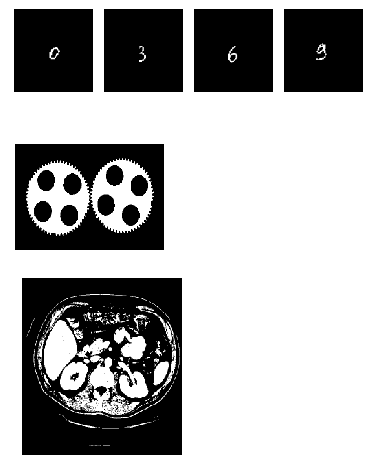
\includegraphics[height=0.8\textheight]{img/34-app.png}
}

\frame {
	\frametitle {İşlemler}

	\begin{itemize}
		\item arkaplandan ve diğerlerinden nesneyi ayırmak

		\item her bir nesneye ait pikselleri bir araya getir

		\item her bir nesne için öznitelikleri hesapla
	\end{itemize}
}

\frame {
	\frametitle{Örnek: kırmızı kan hücreleri}

	\begin{columns}
		\column{0.5\textwidth}
			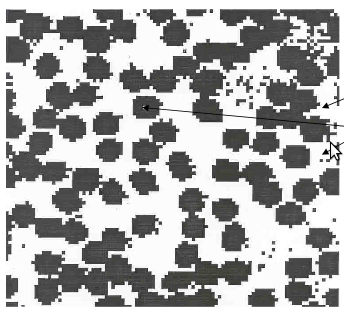
\includegraphics[width=0.9\textwidth]{img/36-cell.png}
		\column{0.5\textwidth}
			\begin{itemize}
				\item çok sayıda ayrı nesne var

				\item bazıları birbirine dokunuyor - kötü! - ayır

				\item tuz ve biber gürültüsü var (eşiklemeden gelen) - filtrele

				\item bu veriden nasıl faydalanılabilir?
			\end{itemize}
	\end{columns}

	\begin{itemize}
		\item  `63` ayrı nesne algılanmıştır
		\item tek hücre alanı yaklaşık olarak `50`'dir
		\item gürültü spotları var
		\item hüvre pıhtıları
	\end{itemize}
}

\frame {
	\frametitle{Daha denetlenebilir resimler}

	\begin{columns}
		\column{0.5\textwidth}
			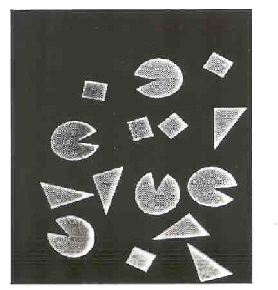
\includegraphics[width=0.9\textwidth]{img/37-pac.png}
		\column{0.5\textwidth}
			\begin{itemize}
				\item daha basit geometrili nesne
				\item daha basit arkaplan
				\item nesneler ayrılabilir durumda
			\end{itemize}
	\end{columns}

	\begin{itemize}
		\item kaç nesne? `15` nesne
		\item nerede?
		\item alanları?
		\item kaç tür?
	\end{itemize}
}

\frame {
	\frametitle{Eşikleme}
	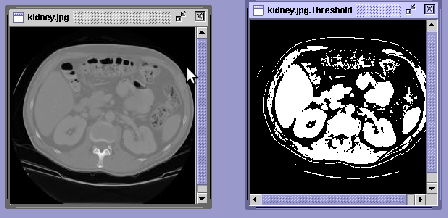
\includegraphics[width=0.9\textwidth]{img/38-thr.png}
	İkil resimler, eşiklemeyle gri resimlerden elde edilebilir.
}

\frame {
	\frametitle{Eşikleme için varsayımlar}

	\begin{itemize}
		\item ilgilendiğimiz nesne arkaplandan farklı bir dağılıma sahip
		olmalıdır

		\item bölgeye ait pikseller, yalnızca parlaklık yardımıyla elde
		edilebilir

		\item :: $parlaklik > T$, $parlaklik < T$ veya $T_1 < parlaklik < T_2$

		\item basit sahnelerde işe yarar

		\item doğal/karmaşık sahnelerde işe yaramaz
	\end{itemize}
}

\frame {
	\frametitle{Eşik seçiminde histogramın kullanımı}

	\begin{columns}
		\column{0.5\textwidth}
			\begin{itemize}
				\item `3` bölgeli kiraz resmi
				\item arkaplan siyah
				\item normal/kaliteli kiraz, parlaktır
				\item çürük kiraz ise orta parlaklıktadır

				\medskip
				\item histogram iki kiraz bölgesini gösterir
			\end{itemize}
		\column{0.5\textwidth}
			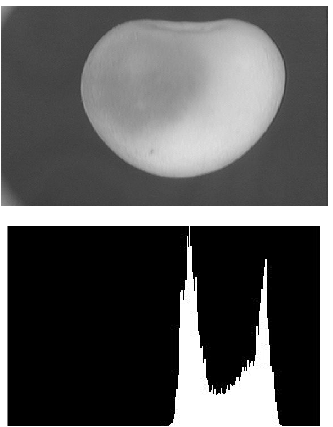
\includegraphics[width=0.9\textwidth]{img/40-thr.png}
	\end{columns}
}

\frame {
	\frametitle{Histogram yönlendirmeli eşikleme}

	bir resimdeki iki veya daha fazla bölgeyi histogram temelinde nasıl
	ayırabiliriz?

	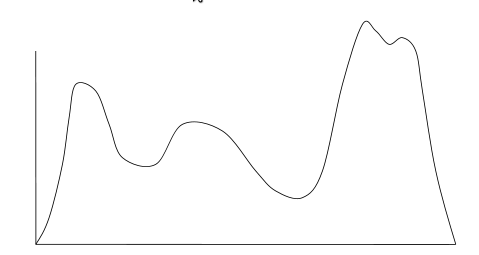
\includegraphics[width=0.9\textwidth]{img/41-hist.png}
}

\frame {
	\frametitle{Eşik Seçimi}

	Tepe ve çukurları algıla
	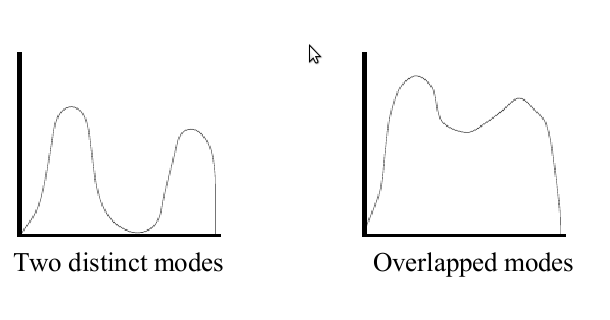
\includegraphics[width=0.9\textwidth]{img/42-cho.png}

	İki farlı mod, örtüşen modlar
}

\frame {
	\frametitle{Eşik Seçimi}

	\begin{itemize}
		\item iki modlu histogramda iki mod arasındaki en derin vadiyi bul

		\item histograma iki veya daha fazla Gauss eğrisi uydur

		\item dinamik eşikleme
	\end{itemize}
}

\frame {
	\frametitle{Eşikleme sonucunda temizlik}

	\begin{columns}
		\column{0.5\textwidth}
			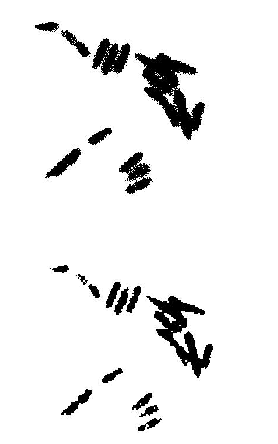
\includegraphics[width=0.9\textwidth]{img/44-cle.png}
		\column{0.5\textwidth}
			\begin{itemize}
				\item daha iyi ayırt etme için sınırdaki nesne piksellerini sil

				\item boşlukları doldur

				\item küçük nesneleri sil

				\item (son ikisi tuz-biber gürültüsüdür)
			\end{itemize}
	\end{columns}
}

\frame {
	\frametitle{Matematiksel Şekilbilim}

	\begin{itemize}
		\item iki temel işlem: \textbf{dilation} ve \textbf{erosion}

		\item ve bunların kombinasyonu: \textbf{opening}, \textbf{closing}, ...
	\end{itemize}
}

\frame {
	\frametitle{Dilation}

	Dilation - genişletme
	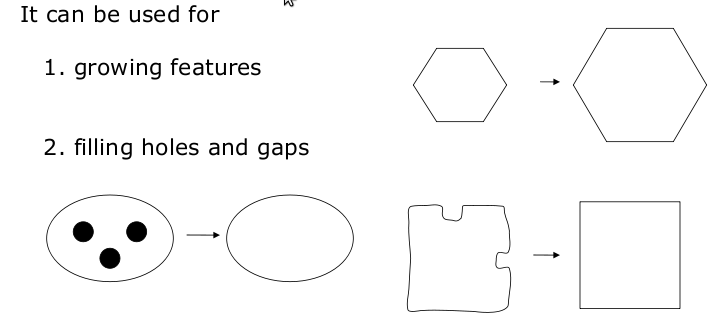
\includegraphics[width=0.9\textwidth]{img/46-dila.png}
}

\frame {
	\frametitle{Erosion}

	Erosion - daraltma
	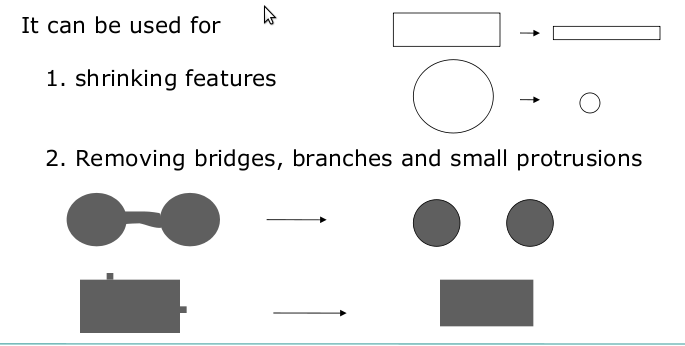
\includegraphics[width=0.9\textwidth]{img/47-ero.png}

	Kan hücre örneğini hatırlayın.
}
\frame {
	\frametitle{Yapı Elemanı}

	\begin{itemize}
		\item yapı elemanı, şekil maskesidir

		\item şekli ve boyutu vardır
	\end{itemize}

	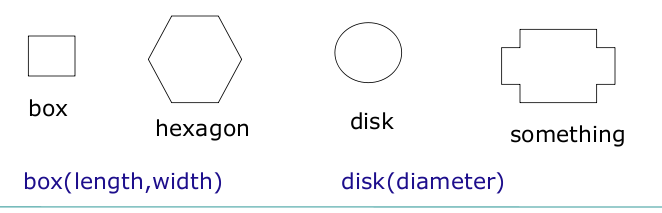
\includegraphics[width=0.9\textwidth]{img/48-str.png}
}

\frame {
	\frametitle{Dilation yapı elemanıyla}

	B: ikil resim ve S: yapı elemanıdır,
	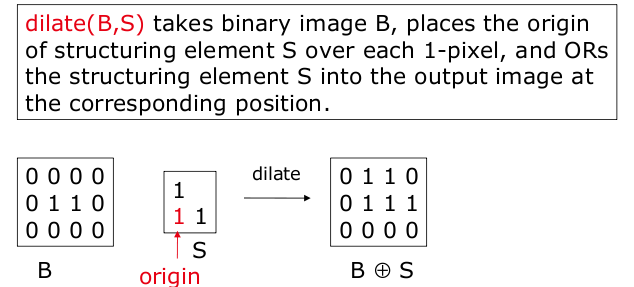
\includegraphics[width=0.9\textwidth]{img/49-dil.png}
}
\frame {
	\frametitle{Dilation}
	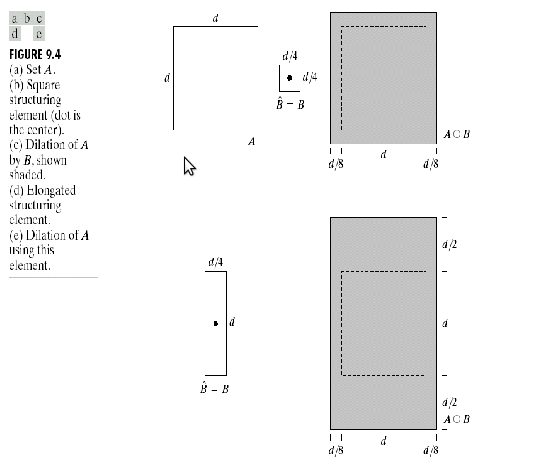
\includegraphics[width=0.9\textwidth]{img/50-dil.png}
}

\frame {
	\frametitle{Dilation}
	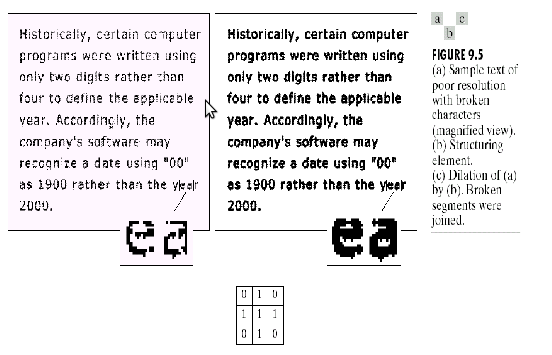
\includegraphics[width=0.9\textwidth]{img/51-dil.png}
}

\frame {
	\frametitle{Erosion yapı elemanıyla}
	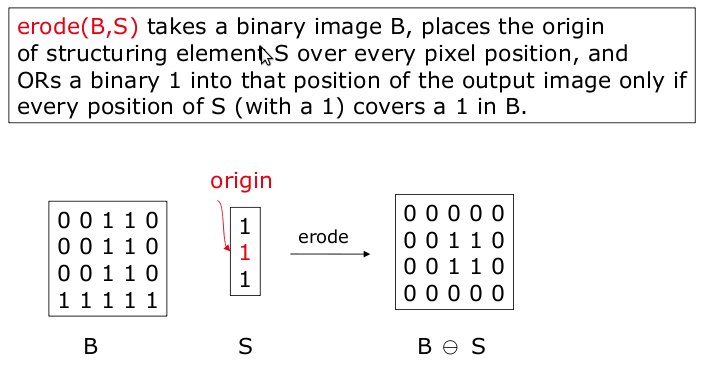
\includegraphics[width=0.9\textwidth]{img/52-ero.png}
}

\frame {
	\frametitle{Erosion}
	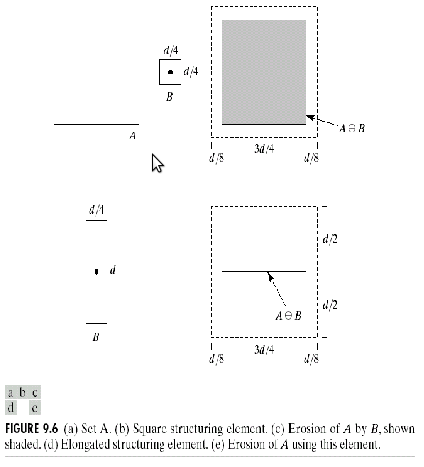
\includegraphics[height=0.8\textheight]{img/53-ero.png}
}

\frame {
	\frametitle{Erosion}
	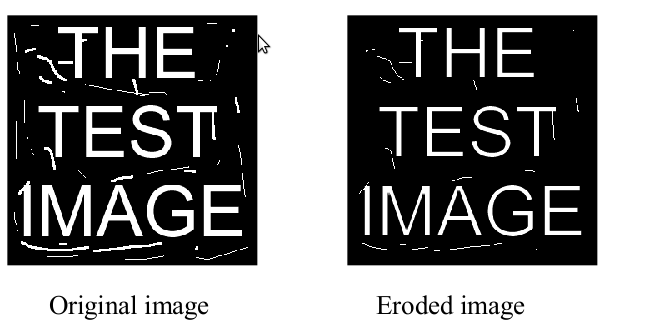
\includegraphics[width=0.9\textwidth]{img/54-ero.png}
}

\frame {
	\frametitle{Erosion}
	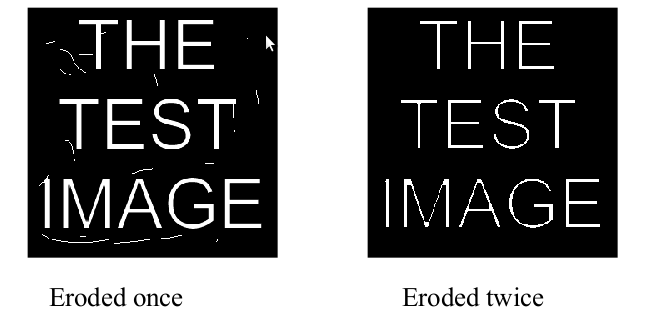
\includegraphics[width=0.9\textwidth]{img/55-ero.png}
}

\frame {
	\frametitle {Opening ve Closing}

	\begin{itemize}
		\item closing: önce erosion sonra dilation
		\item opening: önce dilation sonra erosion
	\end{itemize}
}

\frame {
	\frametitle {Opening ve Closing}

	\begin{itemize}
		\item opening: nesnenin kontörlerini yumuşatır
			$A \circ B  = (A \ominus B) \oplus B$

		\item closing: kontörleri yumuşat; boşlukları doldur

			$A \bullet B = (A \oplus B) \ominus B$

		\item `bwmorph`'ı kurcalayın.
	\end{itemize}
}

\frame {
	\frametitle{örnek 1}
	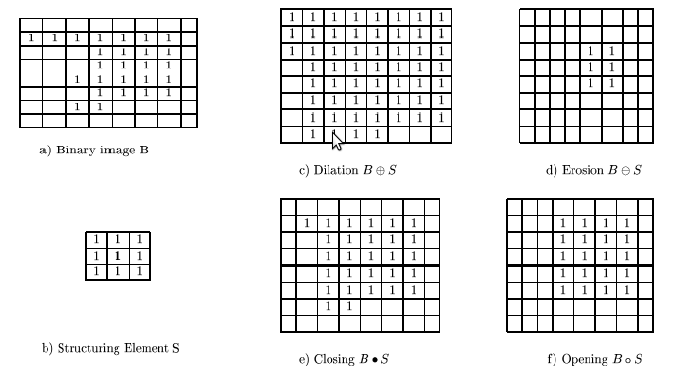
\includegraphics[width=0.9\textwidth]{img/58-ex.png}
}

\frame {
	\frametitle{örnek 1: deneme}
	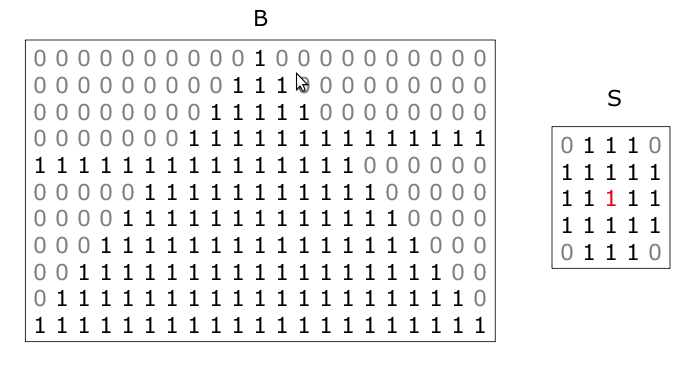
\includegraphics[width=0.9\textwidth]{img/59-try.png}
}

\frame {
	\frametitle{Opening ve Closing}

	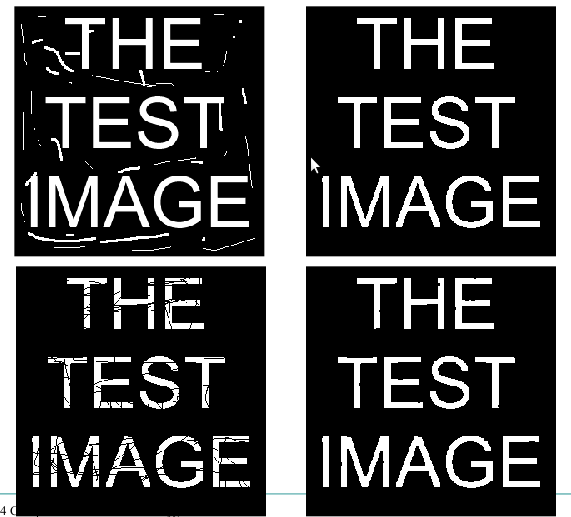
\includegraphics[height=0.8\textheight]{img/60-open.png}

	OPENING: 2xeroded + 2xdilated; gürültüden kurtulduk
	CLOSING: dilated + eroded; boşluklar dolduruldu
}

\frame {
	\frametitle{Opening ve Closing}

	\includegraphics[width=0.9\textwidth]{img/61-open.png}
}

\frame {
	\frametitle{Sınır Çıkarım}
	\includegraphics[width=0.9\textwidth]{img/62-bound.png}
}

\frame {
	\frametitle{Sınır Çıkarım}
	\includegraphics[width=0.9\textwidth]{img/63-bound.png}
}

\frame {
	\frametitle{Bölge Doldurma}
	\includegraphics[width=0.9\textwidth]{img/64-region.png}
}

\frame {
	\frametitle{Bağlı Bileşen Etiketleme}

	ikil resmi elde et, bağlı piksel kümesini belirle ve analiz et

	bağlı bileşen işlemleri, ikil resim alır ve etiket resmini döndürür.
	Değerler `0` ve pozitif tamsayılardır.

	\includegraphics[width=0.9\textwidth]{img/65-conn.png}
}

\frame {
	\frametitle{Bağlı Bileşen Ayrıştırma}

	\includegraphics[width=0.9\textwidth]{img/66-conn.png}
}

\frame {
	\frametitle{sözde renklendirme olarak etiketleme}
	\includegraphics[width=0.9\textwidth]{img/67-label.png}
}

\frame {
	\frametitle{Bağlanırlık}
	\includegraphics[width=0.9\textwidth]{img/68-conn.png}

	4-lü ve 8-li komşuluk
}

\frame {
	\frametitle{Özyineli etiketleme}
	\includegraphics[width=0.9\textwidth]{img/69-rec.png}
}

\frame {
	\frametitle{İlk adım: RLC}
	benzer piksel gruplarına her bir resim satırlarını bölütle (bunlara run
	denir)

	her bir run, sürekliliğe sahip renk değerlerini içeren satırın başlangıç ve
	bitimini saklar

	\includegraphics[width=0.9\textwidth]{img/70-rlc.png}
}

\frame {
	\frametitle{İkinci adım: bölgeleri birleştir}
	\includegraphics[width=0.9\textwidth]{img/71-merge.png}
}

\frame {
	\frametitle{Sonuçlar}

	runlar, çok satırlı bölgelerde birleştirildi

	pikseller yerine resim, sürekliliğe sahip bölgeleri tanımlıyor
	\includegraphics[width=0.9\textwidth]{img/72-res.png}
}

\frame {
	\frametitle{Blob Özellikleri}

	\begin{itemize}
		\item bloblarla ne yapacağız?

		\item hesaplar neler olabilir?

		\item alan/perimeter/oran
		\item kütle merkezi/elips/ortalama renk değeri
		\item vs

		\item bunlar blobu sınıflandırmada yardımcı olabilir
	\end{itemize}
	\includegraphics[width=0.3\textwidth]{img/73-blob.png}
}

\frame { \frametitle{çembersellik} \includegraphics[width=0.9\textwidth]{img/77-cir.png}}
\frame { \frametitle{bounding box} \includegraphics[width=0.9\textwidth]{img/78-bbox.png}}

\frame {
	\frametitle {resim momentleri}

	$M_{ij} = \sum_i \sum_j x^i y^j I(x,y)$

	örneğin $M_{00}$ alanı verirken,
	$(M_{10} / M_{00}, M_{01}/M_{00})$ merkezi verir

	Matlab'da `immoment(im, i, j)`
}

\end{document}
